\section{Fluorescence Life-Time Measurement (FLIM)}

\subsection{Lebenszeit von CFP und YFP}

\subsubsection{Methode 1: Fit}
In diesem Versuchsteil geht es um die Bestimmung der Lebensdauer des Donors und des Akzeptors. Dies tut man am 
besten indem man eine einfache Exponentialfunktion an die Daten anpasst. Dabei passt man zwei Parameter an, die Amplitude $A_0$ und 
Lebensdauer $\tau$.

\begin{equation}
    A(t) = A_0 \cdot \exp(-\frac{t}{\tau})
\end{equation}

Aus den einzelnen Parametern der angepassten Exponentialfunktionen bildet man dann den Mittelwert. Das es jeweils für CFP und YFP 9 Werte gibt, 
verkleinert sich der Fehler um einen Faktor drei.\\
Aus den Anpassungen erhält man folgende Werte:\\

\begin{center}
    \centering
    \begin{tabular}{l|cr}
        \toprule
        Messung & Lebensdauer CFP (ns)& Lebensdauer YFP (ns)\\
        \midrule
        Kanal 1 & 2,4985& 3,0513\\
        Kanal 1 & 2,5074& 3,0670\\
        Kanal 1 & 2,5623& 3,0482\\
        \midrule
        Kanal 2 & 2,5483& 3,0482\\
        Kanal 2 & 2.4853& 3,1066\\
        Kanal 2 & 2,5123& 3,0923\\
        \midrule
        Kanal 1\&2 & 2,5458& 3,0923\\
        Kanal 1\&2 & 2,5063& 3,0682\\
        Kanal 1\&2 & 2,5595& 3,0500\\
        \midrule
        Mittelwert & 2,5251& 3,0693\\
        Fehler& 0,0036& 0,0043\\
        Ergebnis:& \textcolor{red}{2,5251 $\pm$ 0,0012}& \textcolor{red}{3,0693 $\pm$ 0,0043}\\
        \bottomrule
    \end{tabular}
\end{center}

Man sieht also einen Unterschied in der Lebenszeit der beiden Proteine. Der eigentlich spannende Teil 
ist jedoch die Lebensdauer des Donators mit und ohne FRET zu vergleichen.

\subsubsection{Methode 2: Maximum-Likelihood-Methode}

Die Maximum-Likelihood-Schätzung \cite[S.176]{Stahel2000} ist eine Methode bei der man einen maximal wahrscheinlichen Parameter schätzt.
Dieser ist dann anhand der Daten der plausibelste Parameter. Nun ergibt sich für die Lebensdauer nach der
ML-Methode, dass der beste Schätzer der arithmetischem Mittelwert der Zerfälle ist.
Wendet man diese an erhält man nach der Formel

\begin{equation}
    \tau = \frac{1}{N} \sum_i^N t_i
\end{equation}

wobei $N$ die Anzahl der verwendeten Datenpunkte und $t$ die Zerfallszwit sind. Leider hat diese Methode hier auf Grund 
eines Umsetzungsfehlers nicht funktioniert, da der erhaltene Wert unsinnig ist. Wir haben für 

\begin{equation*}
    \tau_{YFP} = 179,31\,ns
\end{equation*}
erhalten. 



\subsection{Lebensdauer mit FRET}

Um die FRET-Effizienz $E$ zu erhalten, betrachtet man Lebensdauerunterschiede des Donor mit und ohne FRET. 
Man erwartet eine Verkürzung der Lebensdauer $\tau_D$ des Donator bei hinzukommen von FRET. Um es vorweg zu nehmen: Die Methode funktioniert hier sehr schlecht. 
Man versucht das zu bewerkstelligen, indem man eine Anpassung zweier Exponentialfunktionen macht. Diese beinhalten dann insgesamt 4 Parameter; 
ein Fit mit 4 Parametern ist jedoch sehr störungsanfällig.\\

Deswegen verwenden wir eine Methode, bei der wir jeweils zwei Parameter anpassen und die anderen gleich lassen. Danach passt man die anderen zwei 
Parameter schrittweise an. Dieses Vorgehen führt zu einer schrittweisen Approximation, da sich beide Parameter ihrem Maximum annähern. Mit dieser 
Methode erhält man die Werte, welche in Tabelle \ref{LTFit} dargestellt werden. Dabei werden die ersten zwei Werte für die Lebenszeit von den einzelnen Fits der CFP und YFP Probe genommen.\\

\begin{table}[h]
    \centering
    \begin{tabular}{l|rr||rr}
        \toprule
        Schritt & $\tau_{YFP}$ & $A_{0_{YFP}} $&  $\tau_{CFP}$ & $A_{0_{CFP}}$\\
        \midrule
        1 & 3,0693\,ns & & 2,5351\,ns& \\
        2 & & 93514,30\,$s^{-1}$ & & 15228,19 \,$s^{-1}$\\
        3 & 2,8911\,ns & & 3,6229\,ns& \\
        4 & & 94794,70\,$s^{-1}$ & & 14407,05 \,$s^{-1}$\\
        5 & 2,8791\,ns & & 3,6991\,ns& \\  
        \bottomrule
    \end{tabular}
    \caption{Schrittweises Anpassen zweier Exponentialfunktionen an die Daten. Es werden immer zwei Parameter festgehalten. Die anderen zwei werden 
    angepasst.}
    \label{LTFit}
\end{table}

Aus dieser kann man dann die FRET-Effizienz berechnen indem man die Formel 
\begin{equation}
    E = 1 - \frac{\tau_{CFP, FRET}}{\tau_{CFP, NoFRET}}
\end{equation}
auswertet. Dabei erhält man als Ergebnis den Werte 
\begin{equation}
    \textcolor{red}{E = 1 - \frac{3,6994\,ns}{2,5251\,ns} = −0,46}, 
\end{equation}
welcher offensichtlich unsinnig ist. \\
Die Methode scheint also nicht zu funktionieren. Ein Grund dafür könnte die Anzahl der anzupassenden Parameter 
sein. Dabei können einzelne Parameter in den Hintergrund treten, während andere mehr gewicht erhalten. So erhält man ein verfälschtes Fitergebnis.

\clearpage
\subsection{Impulsantwort}

Im folgenden Abschnitt wollen wir die Impulsantwort des Systems charakterisieren. Dazu verwenden wir Kanal 1 bei der YFP Probe. Dabei wird das auf zwei Arten gemacht. 
Die erste Art ist sich die Impulsantwort (IRF) durch das Programm 'SymPhoTime' ausgeben zu lassen. Dieses berechnet die IRF in dem 
sie das Signal entfaltet. Die andere Variante ist es eine Gaußkurve an das Histogram anzupassen. Diese wird der IRF entsprechen, 
weil wir von einer abgeschnittenen Exponentialfunktion ausgehen als ideales Signal.\\
Allgemein beginnen wir mit der Betrachtung des Histograms der Lebensdauer der Einzelphotonenereignisse. Dabei fällt auf, dass es eine Totzeit des 
Detektors gibt. Diese ist sehr schön in der Abbildung \ref{bild:IRFGaussian} zu sehen.\\
\begin{figure}[h]
    \centering
    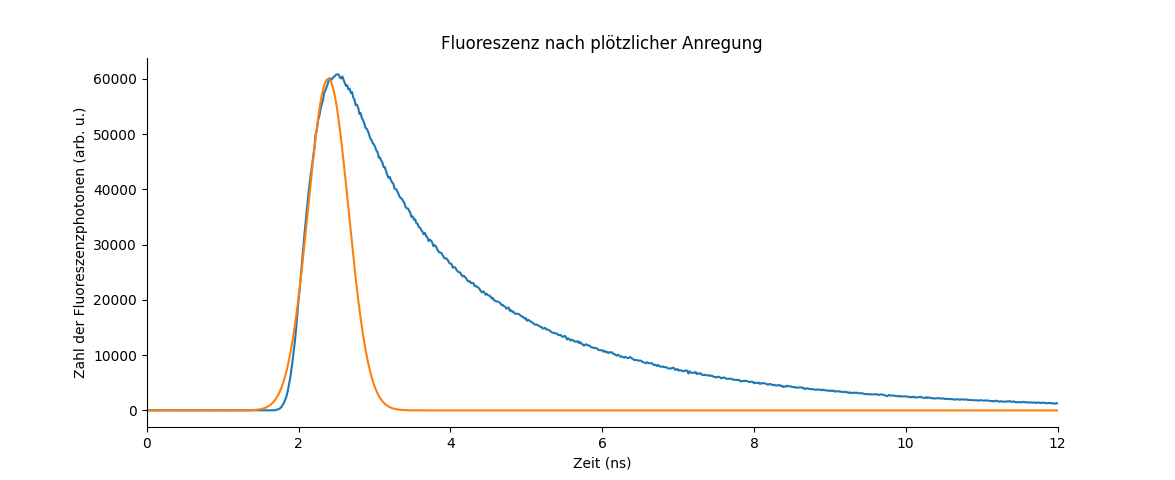
\includegraphics[width = \linewidth]{Bilder/Auswertung/IRFGaussian.png}
    \caption{Lebensdauer bei Einzelphotonenereignissen. Als Probe wurde YFP verwendet und gemessen wurde im Bereich 535-585\,nm. Schön zu sehen ist die Totzeit des Detektors am Anfang. 
    An die Daten wurde eine Gaußfunktion angepasst um die IRF zu charakterisieren.}
    \label{bild:IRFGaussian}
\end{figure}

Wie lange die Totzeit genau ist, ist relativ schwer zu sagen. Aber man kann sie grafisch abschätzen. Sie liegt vermutlich im Anstieg 
der Kurve. Genau abzulesen wo diese ist, geht nicht daher schätzen wir, dass\\

\begin{equation*}
    \textcolor{red}{t_{tot} = (2,0\pm0,5)\,ns}
\end{equation*}

ist. Der Fehler ist jedoch relativ groß. \\
Dann passen wir wie in Abbildung \ref{bild:IRFGaussian} zu sehen, eine Gaußfunktion an diese an. Diese Falten wir dann mit der bei 2 
abgeschnittenen Exponentialfunktion. Das Ergebnis liegt schon nahe an dem wirklichen Daten, wie in Abbildung \ref{bild:IRFconvGauss} zu sehen; aber es kann noch verbessert werden, indem man den Parameter $\tau_{YFP}$ variiert, da dieser auch bei Fit schon 
durch die IRF verzerrt wurde. Dazu gibt es mehrere Möglichkeiten. Man kann eine Cost-Funktion aufstellen, also eine Funktion die den Squared-Error angibt und diese 
dann minimieren. Dies hat den Nachteil, dass diese Methode anfällig für Fehler ist. Es können sich beispielsweise kleine Fehler in höheren 
Teilen des Spektrum sich aufaddieren können. Wenn man optisch die Funktion anpasst, hat das den Vorteil, dass man nicht die allgemeine Steigung aus dem Auge 
verliert, indem man nicht nur auf die Fehler schaut. Deswegen ist diese Methode hier zu bevorzugen.\\

\begin{figure}[h]
    \centering
    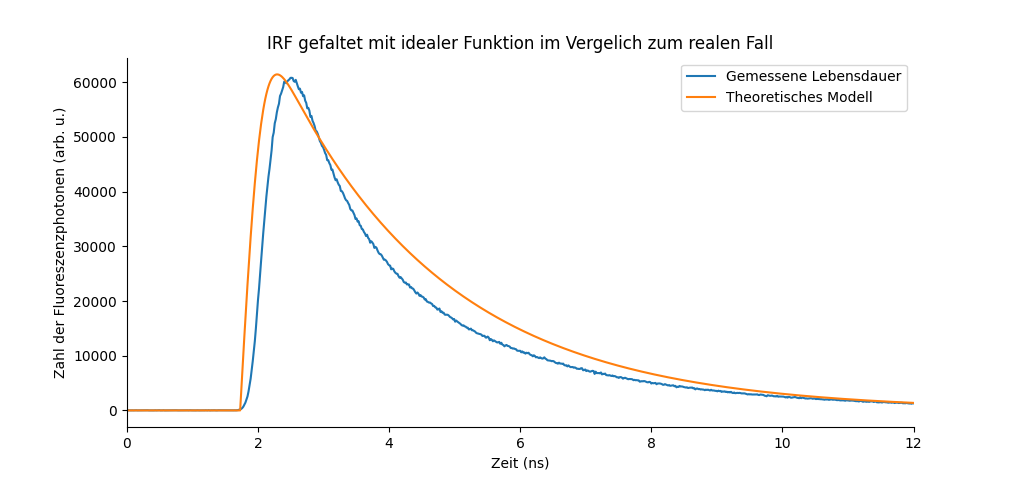
\includegraphics[width = \linewidth]{Bilder/Auswertung/IRFGaussianConvol.png}
    \caption{Lebensdauer bei Einzelphotonenereignissen und die Faltung der IRF und dem idealen Signal nach der Totzeit. Das (nicht dargestellte) ideale Signal ist in diesem 
    Modell noch verzerrt, da es mit den Daten, welche die IRF beinhalten, noch gefittet wurde.}
    \label{bild:IRFconvGauss}
\end{figure}

Durch manuelles Anpassen der Lebensdauer des YFP auf 

\begin{equation*}
    \tau_{YFP} = 2,1
\end{equation*}

erhält man einen realistischeren Wert. Dieser ist jedoch mit einer großen Unsicherheit behaftet, da weder die IRF wirklich wie eine 
Gaußfunktion aussehen muss noch die Totzeit 2\,ns betragen muss. Daher nehmen wir 
\begin{equation*}
    \textcolor{red}{\tau_{YFP} = (2,1\pm0,4)\,ns}
\end{equation*}
als realistischen Wert an. Dieser passt bei beiden Methoden, dem Gaußfit und der programmgenerierten IRF (siehe Abb. \ref{bild:IRFProg}), wie man in den optimierten Abbildungen \ref{bild:IRFconvGaussOpt} und \ref{bild:IRFconvProOpt} sieht.
Tut man eben dies mit einer Cost-Funktion wie in Abbildung \ref{bild:Cost} zu sehen erhält man näherungsweise den selben Wert. Dabei ist der lineare Verlauf der Funktion sehr unerwartet.

\begin{figure}[h]
    \centering
    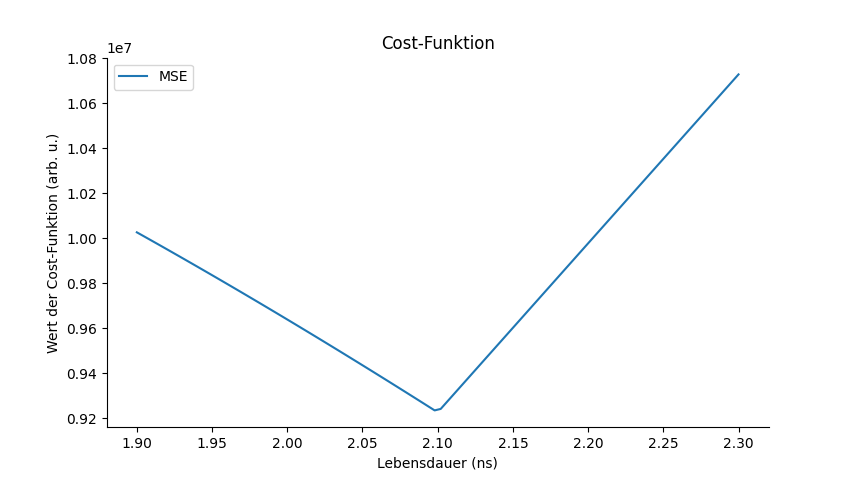
\includegraphics[width = \linewidth]{Bilder/Auswertung/Cost.png}
    \caption{Cost-Funktion zum Finden der realen Lebenszeit von YFP}
    \label{bild:Cost}
\end{figure}



\begin{figure}[h]
    \centering
    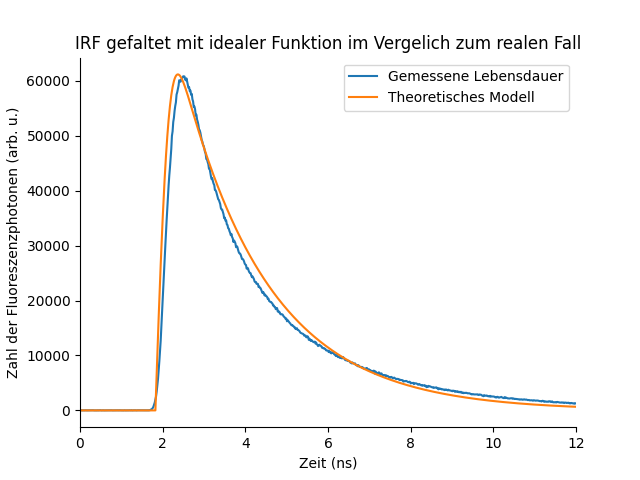
\includegraphics[width = \linewidth]{Bilder/Auswertung/IRFGaussianConvolCorrectet.png}
    \caption{Lebensdauer bei Einzelphotonenereignissen und die Faltung der IRF und dem idealen Signal ($\tau_{YFP}$ optimiert) nach der Totzeit. Es zeigt sich, dass die theoretische Kurve 
    den Sachverhalt nun besser beschreibt als in Abbildung \ref{bild:IRFconvGauss}}
    \label{bild:IRFconvGaussOpt}
\end{figure}

\begin{figure}[h]
    \centering
    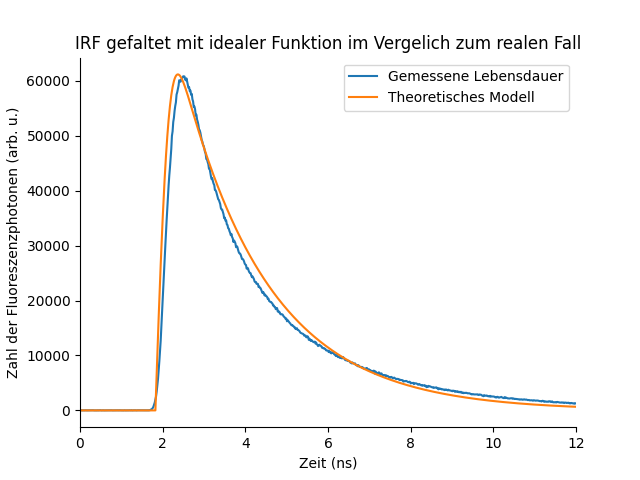
\includegraphics[width = \linewidth]{Bilder/Auswertung/IRFGaussianConvolCorrectet.png}
    \caption{Lebensdauer bei Einzelphotonenereignissen und die Faltung der IRF und dem idealen Signal ($\tau_{YFP}$ optimiert) nach der Totzeit. Es zeigt sich, dass die theoretische Kurve 
    den Sachverhalt nun besser beschreibt als in Abbildung \ref{bild:IRFconvProg}}
    \label{bild:IRFconvProOpt}
\end{figure}


